\documentclass{scrreprt}

\usepackage{graphicx}
\usepackage{tikz}
\usepackage{amstext}
\usepackage{hyperref}
\usepackage{amsfonts}
\usepackage{tabularx}
\usepackage{multirow}
\usepackage{amssymb}
\usepackage{textcomp}
\newcommand\tab[1][1cm]{\hspace*{#1}}

\hypersetup{
  colorlinks=false,
  linkbordercolor=blue,
  pdfborderstyle={/S/U/W 0}
}
\title{\textbf{Algorithmen und Datenstrukturen}}
\author{\href{https://github.com/bircni}{\color{blue}github/bircni}}
\date{\href{https://ko-fi.com/toiletcoders}{\color{black}little donation}}
\begin{document}
\pagenumbering{gobble}
\maketitle
\pagebreak
\renewcommand{\contentsname}{Inhaltsverzeichnis}
%\renewcommand{\cftdot}{}
\setcounter{tocdepth}{1}
\tableofcontents
\addtocontents{toc}{~\hfill\textbf{Seite}\par}
\pagebreak
\pagenumbering{arabic}
\chapter{Mathematische Grundlagen}
\section{Reihen}
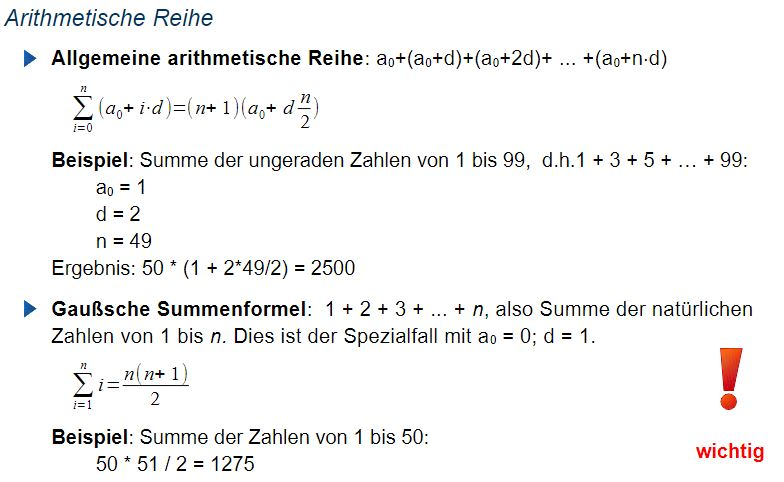
\includegraphics[width=0.7\textwidth]{graphics/reihen-arithmetisch}
\section{Potenzen und Logarithmen}
Der Logarithmus ist die Inverse der Potenzfunktion. $\log_a(x) = y \quad \Longleftrightarrow  \quad a^y = x$
\\\textbf{spezielle Logarithmen:}
\\$ld(x)=log_2(x)$, $lg(x)=log_10(x)$, $ln(x)=log_e(x)$
\section{Notationskonventionen}
$\lceil x \rceil$ zur nächsten ganzen Zahl aufrunden
\\$\lfloor x \rfloor$ zur nächsten ganzen Zahl abrunden
\\$[a .. b] = {x \arrowvert a \leq x \wedge x \leq b}$ mit Intervallgrenzen
\\$]a .. b[ = {x \arrowvert a < x \wedge x < b}$ ohne Intervallgrenzen
\\$arr[i .. k]$ Teilfolge der Elemente von $arr[i]$ bis $arr[k]$

%2.4:
\end{document}